Un ejemplo de respuesta en lenguaje natural se vio en el Listado~\ref{lst:APIresponse2}. En el Listado~\ref{lst:APIresponse1} se muestra (simplificada) la respuesta recibida en el caso de la consulta del día en curso (\textcopyright AEMET).
\begin{lstlisting}[numbers=none,float=ht,caption={Ejemplo de respuesta de la API-AEMET para el día en curso},label={lst:APIresponse1}]
{
 origen: {
	productor: "Agencia Estatal de Meteorología - AEMET. Gobierno de España",
	web: "http://www.aemet.es",
	language: "es",
	copyright: "AEMET. Autorizado el uso de la información y su reproducción citando a AEMET como autora de la misma.",
	notaLegal: "http://www.aemet.es/es/nota_legal"
 },
 elaborado: "2019-2-12",
 nombre: "Consuegra",
 provincia: "Toledo",
 prediccion: {
 	dia: [
		{
		 estadoCielo: [
					{
					 periodo: "08",
					 descripcion: "Cubierto"
					},
					{
					 periodo: "09",
					 descripcion: "Cubierto con lluvia escasa"
					},
					{
					 periodo: "10",
					 descripcion: "Cubierto con lluvia escasa"
					},
					{
					 periodo: "11",
					 descripcion: "Cubierto"
					},
					...
		 ]
		}
	}
}
\end{lstlisting}
\\

Cómo se puede observar se diferencia de la respuesta en texto del Listado~\ref{lst:APIresponse2}, pues se trata de una respuesta \gls{JSON}, que es un formato de texto simple que se utiliza para el intercambio de información, aunque tuvo sus inicios en Javascript, haciendo honor a su nombre (\textit{Javascript Object Notation}).\\
En el campo 'predicción' existe un subcampo 'estadoCielo' (entre otros que se han obviado por no ser de interés en este trabajo) que contiene una lista con los estados meteorológicos de la previsión. Cada elemento de la lista contiene dos valores: periodo (hora del día de esa previsión) y descripción (cadena de texto que describe el estado del cielo, mismo conjunto de palabras que se emplea para encontrar las ocurrencia en el texto en el otro tipo de respuesta). Claramente existe un problema con los conjuntos de estados meteorológicos que se obtienen de procesar las peticiones a la \gls{API} \gls{AEMET}, ya que para la determinación de la máxima energía fotovoltaica posible en una hora t debe conocerse \gls{CMP}, la potencia nominal posible (potencia que es capaz de suministrar el módulo fotovoltaico), directamente proporcional al estado meteorológico, el cuál es un texto que describe la situación y no un valor numérico que representa los watios que puede dar un módulo en esas condiciones, y a priori no se dispone de una forma directa de relacionarlas. Por tanto, se emplea \textbf{lógica difusa} para resolver la problemática mencionada anteriormente.
\subsection{Lógica difusa}
La teoría de la lógica difusa proporciona un marco matemático que permite modelar la incertidumbre de los procesos cognitivos humanos para poder ser tratable por un computador. Estos procesos cognitivos hacen referencia a expresiones del tipo:
\begin{itemize}
	\item Si no vives \textit{lejos} puedes ir en bicicleta.
	\item Si hace \textit{mucho} frío llévate un chaquetón.
\end{itemize}
Los humanos son capaces de interpretar estos valores rápidamente. Sin embargo, las máquinas no tienen esa capacidad, debido a que no existe un valor cuantitativo que indique la distancia a la que se refiere la palabra \textit{lejos} o que temperatura es \textit{mucho} frío. Si se intentan trasladar estas reglas a código, aparecen dificultades ya que no se puede procesar numéricamente. Una opción es definir intervalos de valores que comprenderá cada palabra (por ejemplo, tomando \textit{lejos} como la distancia comprendida entre 5 y 10 kilómetros), pero esto no es preciso ya que para un computador, la distancia de 5,01 kilómetros sería igual de lejos que 9,9 kilómetros, cuando en realidad la interpretación correcta no es así. Con esto queda a la vista que la lógica convencional no trata de forma eficiente este problema presentando numerosas limitaciones. Otro ejemplo típico es el mostrado en la Figura~\ref{fig:ejemplo_logica}, donde se puede observar como la lógica clásica interpretaría erróneamente el hecho: \textit{Una persona de dos metros es alta}, pues clasificaría una persona de 1,99 metros como no alta, mientras que la lógica difusa lo clasificaría mediante un grado de pertenencia. La solución pasa por emplear un método de razonamiento afín a la lógica difusa.\\
\begin{figure}[!h]
	\centering
	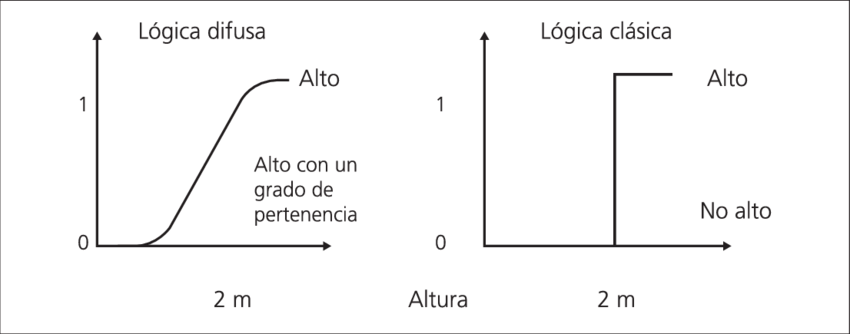
\includegraphics[width=9cm]{figs/tipos_logica.png}
	\caption{Lógica clásica vs. lógica difusa}
        \label{fig:ejemplo_logica}
\end{figure}

La lógica difusa~\cite{Morc11} permite representar matemáticamente la \textbf{incertidumbre}. Según Zadeh~\cite{Zad73}, "\textit{Cuando aumenta la complejidad, los enunciados precisos pierden su significado y los enunciados útiles pierden precisión.}", es decir, \textit{los árboles no te dejan ver el bosque}, pues prácticamente cualquier problema del mundo puede resolverse partiendo de unas variables de entrada y buscando obtener como objetivo un conjunto de variables de salida. La lógica difusa establece esta relación entre variables de forma correcta.

\subsection{Conjuntos difusos}
En la teoría de conjuntos de la lógica clásica, el grado de pertenencia puede tomar solo los valores 0 y 1, que representan que el elemento pertenece o no pertenece al conjunto. En la lógica difusa existe el concepto de \textbf{conjunto difuso}~\cite{Zad65}, establecido por Zadeh. Para trabajar con valores difusos se realiza un proceso denominado \textit{fuzzificación} que da resultados difusos. Estos resultados se someten a un proceso de \textit{defuzzificación} para transformarse en valores discretos (llamados \textit{crisp}), que tendrán un \textbf{grado de pertenecia} a los conjuntos difusos el cuál será un valor en el intervalo [0, 1], y representa cuanto pertenece al conjunto.\\

Así pues, hay un claro ejemplo de conjuntos difusos con los estados meteorológicos. En la Figura~\ref{fig:estadoCielo} se muestran los estados meteorológicos que proporciona la \gls{API} de \gls{AEMET}~\cite{Aemet} (Obtenida de la web oficial de \textcopyright AEMET).
\begin{figure}[H]
	\centering
	
\includegraphics[width=17cm]{figs/estadoCieloAEMET.png}
	\caption{Posibles estados del cielo en AEMET}
	\label{fig:estadoCielo}
\end{figure}
Como se puede observar existe un gran número de estados meteorológicos, y en muchos de ellos un módulo fotovoltaico no genera energía. En estos estados el valor máximo a generar por los módulos será de 0 watios. Los estados favorables (donde un módulo genera una potencia mayor a 0 watios) serán representados como conjuntos difusos. En la Tabla~\ref{tab:estadosFavorables} se muestran cuáles son estos estados. Por ejemplo, no se puede determinar cuantos watios se producen como máximo con un tiempo \textit{Despejado} o \textit{Cubierto con nubes altas}, pero podemos mostrar los conjuntos difusos y gráficamente comprobar su distribución, para obtener un valor discreto de cada conjunto difuso, denominado \textbf{centroide} o centro de gravedad del conjunto difuso. Este proceso es conocido como razonamiento aproximado a partir de inferencia difusa. La inferencia difusa permite obtener un valor de salida para un valor de entrada empleando la teoría de conjuntos difusos. Un ejemplo de cuestión a resolver es: \textit{¿Qué potencia pico se puede obtener de un módulo fotovoltaico si hay intervalos nubosos?}. Cómo hemos comentado anteriormente, la respuesta sería el centroide del conjunto difuso \textit{Intervalos Nubosos}. El centroide es el punto que divide el conjunto difuso en dos partes de igual masa. En la Ecuación~\ref{eq:centroide} se muestra el procedimiento para calcularlo, realizando el sumatorio de las potencias tomadas por su grado de pertenencia al conjunto dividido entre el sumatorio de dichos grados de pertenencia. En la Tabla~\ref{tab:estadosFavorables} se incluye el valor del centroide de cada etiqueta lingüistica.\\
\begin{equation}
        \label{eq:centroide}
        Centroide = \frac{\sum_{x=i}^{n} x \mu_{A}(x)}{\sum_{x=i}^{n} \mu_{A}(x)}
\end{equation}
Para representar las variables lingüisticas, se parte del hipotético caso en el que cada variable desciende de manera ligeramente más inclinada que asciende, representando el factor de adaptación de un módulo fotovoltaico a un nuevo estado meteorológico. En la Figura~\ref{fig:fuzzySets} se pueden observar las variables lingüisticas definidas en la Tabla~\ref{tab:estadosFavorables}. En el eje horizontal se encuentra la potencia máxima que puede generar el módulo fotovoltaico en watios y en el eje vertical el grado de pertenencia a cada variable en el intervalo [0,1]. Si se avanza en el eje horizontal, se observa que el estado meteorológico es cambiante hacia estados favorables, y viceversa, ya que esto es directamente proporcional a la máxima potencia posible generada por el módulo.

Cada conjunto difuso es una función PI o \textbf{trapezoidal}, ya que no existe un único punto donde el grado de pertenencia al conjunto es 1, si no que se mantiene ese valor de pertenencia hasta que el módulo comienza a experimentar un cambio en el estado del cielo y se debe adaptar a dicho estado.

\begin{figure}[h]
	\centering
	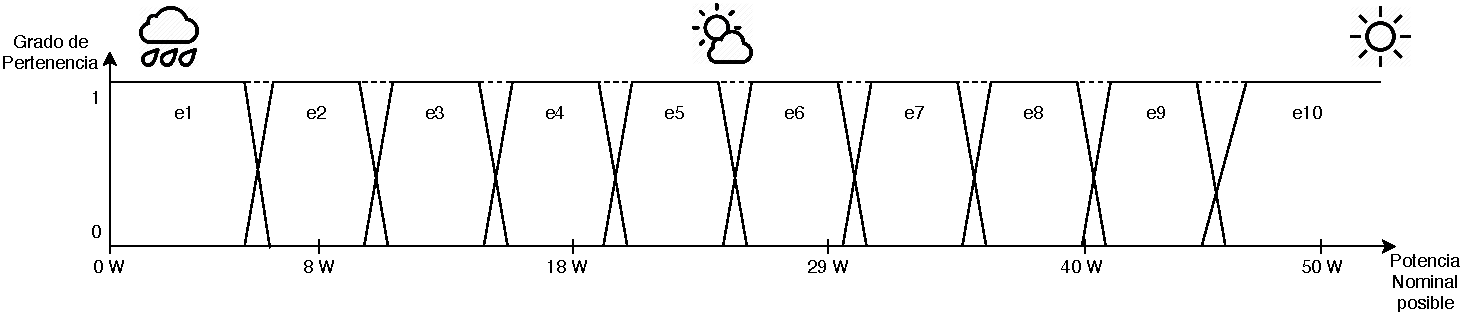
\includegraphics[width=17cm]{figs/Fuzzy_diagram.pdf}
	\caption{Conjuntos difusos de los estados meteorológicos}
        \label{fig:fuzzySets}
\end{figure}

Tal y cómo se comentó en la iteración anterior, se utilizan módulos fotovoltaicos con \gls{CMP} de 50 watios, que solo podría ser alcanzada en el estado meteorológico óptimo (\textit{Despejado}), y en función de este dato, se toman los valores para obtener los centroides.
\begin{table}[H]
        \centering
        \begin{tabular}{|c|l|c|}
                \hline
                \textbf{Etiqueta lingüistica} & \textbf{Descripción} & \textbf{Centroide} \\ \hline
                e10 & Despejado & 48 W \\ \hline
                e9 & Poco nuboso & 43,16 W \\ \hline
                e8 & Nubes altas & 38,16 W \\ \hline
                e7 & Intervalos nubosos & 33,16 W \\ \hline
                e6 & Intervalos nubosos con lluvia escasa & 28,16 W \\ \hline
                e5 & Intervalos nubosos con lluvia & 23,16 W \\ \hline
                e4 & Nuboso & 18,16 W \\ \hline
                e3 & Nuboso con lluvia escasa & 13,16 W \\ \hline
                e2 & Cubierto & 8,16 W \\ \hline
                e1 & Cubierto con lluvia escasa & 2,66 W\\ \hline
        \end{tabular}
        \caption{Variable lingüistica de la CMP}
        \label{tab:estadosFavorables}
\end{table}

El dominio de la variable lingüistica es [0, 50] Watios. Estos valores se almacenarán en un diccionario, disponible en el fichero de constantes del proyecto (módulo \textit{project\_constants}). Dicho diccionario será usado para realizar el parseo de los estados meteorológicos obtenidos de la \gls{API} \gls{AEMET} (cadenas de texto) a valores cuantitativos (centroide del conjunto difuso), y poder ser usables por el sistema para determinar la \textbf{máxima energía fotovoltaica} que se puede obtener en un momento determinado.
